\documentclass{article}
\usepackage[margin=1in]{geometry}
\usepackage{amsmath,amsthm,amssymb}
\usepackage{bbm,enumerate,mathtools}
\usepackage{tikz,pgfplots}
\usepackage{chessboard}
\usepackage[hidelinks]{hyperref}
\usepackage{multicol} % Problem 35

\newenvironment{question}{\begin{trivlist}\item[\textbf{Question.}]}{\end{trivlist}}
\newenvironment{note}{\begin{trivlist}\item[\textbf{Note.}]}{\end{trivlist}}
\newenvironment{references}{\begin{trivlist}\item[\textbf{References.}]}{\end{trivlist}}
\newenvironment{related}{\begin{trivlist}\item[\textbf{Related.}]\end{trivlist}\begin{enumerate}}{\end{enumerate}}

\usetikzlibrary{patterns}

\begin{document}
\rating{2}{3}
Consider regions of the plane that can contain all $n$-ominoes up to
dihedral action.

\begin{figure}[ht!]
  \centering
  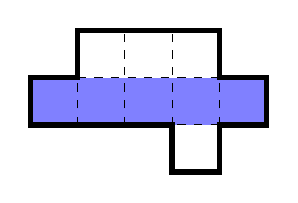
\begin{tikzpicture}[scale=0.6]
    \fill[blue!50] (0,0) rectangle (5,1);
    \draw[line width=2] (0,0)--(3,0)--(3,-1)--(4,-1)--(4,0)--(5,0)--(5,1)--(4,1)--(4,2)--(1,2)--(1,1)--(0,1)--cycle;
    \draw[dashed] (1,0) grid (4,2);
  \end{tikzpicture}
  \hspace{0.5cm}
  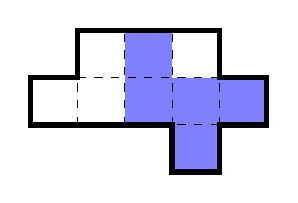
\begin{tikzpicture}[scale=0.6]
    \fill[blue!50] (2,0) rectangle (5,1);
    \fill[blue!50] (3,1) rectangle (4,-1);
    \fill[blue!50] (2,0) rectangle (3,2);
    \draw[line width=2] (0,0)--(3,0)--(3,-1)--(4,-1)--(4,0)--(5,0)--(5,1)--(4,1)--(4,2)--(1,2)--(1,1)--(0,1)--cycle;
    \draw[dashed] (1,0) grid (4,2);
  \end{tikzpicture}
  \hspace{0.5cm}
  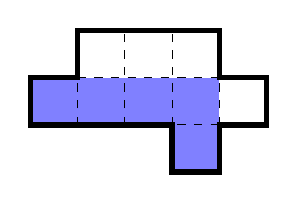
\begin{tikzpicture}[scale=0.6]
    \fill[blue!50] (0,0) rectangle (4,1);
    \fill[blue!50] (3,-1) rectangle (4,1);
    \draw[line width=2] (0,0)--(3,0)--(3,-1)--(4,-1)--(4,0)--(5,0)--(5,1)--(4,1)--(4,2)--(1,2)--(1,1)--(0,1)--cycle;
    \draw[dashed] (1,0) grid (4,2);
  \end{tikzpicture}
  \hspace{0.5cm}
  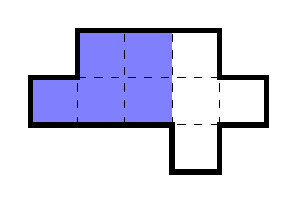
\begin{tikzpicture}[scale=0.6]
    \fill[blue!50] (1,0) rectangle (3,2);
    \fill[blue!50] (0,0) rectangle (2,1);
    \draw[line width=2] (0,0)--(3,0)--(3,-1)--(4,-1)--(4,0)--(5,0)--(5,1)--(4,1)--(4,2)--(1,2)--(1,1)--(0,1)--cycle;
    \draw[dashed] (1,0) grid (4,2);
  \end{tikzpicture}
  \\~\\
  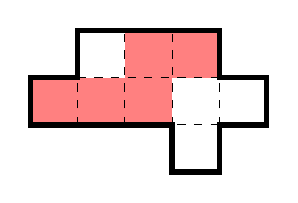
\begin{tikzpicture}[scale=0.6]
    \fill[red!50] (0,0) rectangle (3,1);
    \fill[red!50] (2,0) rectangle (3,2);
    \fill[red!50] (2,1) rectangle (4,2);
    \draw[line width=2] (0,0)--(3,0)--(3,-1)--(4,-1)--(4,0)--(5,0)--(5,1)--(4,1)--(4,2)--(1,2)--(1,1)--(0,1)--cycle;
    \draw[dashed] (1,0) grid (4,2);
  \end{tikzpicture}
  \hspace{0.5cm}
  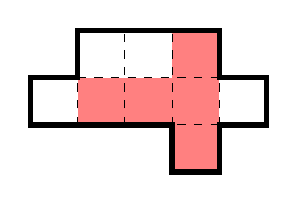
\begin{tikzpicture}[scale=0.6]
    \fill[red!50] (1,0) rectangle (4,1);
    \fill[red!50] (3,-1) rectangle (4,2);
    \draw[line width=2] (0,0)--(3,0)--(3,-1)--(4,-1)--(4,0)--(5,0)--(5,1)--(4,1)--(4,2)--(1,2)--(1,1)--(0,1)--cycle;
    \draw[dashed] (1,0) grid (4,2);
  \end{tikzpicture}
  \hspace{0.5cm}
  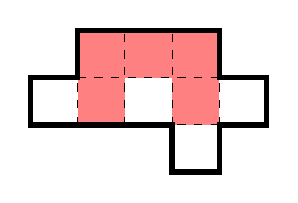
\begin{tikzpicture}[scale=0.6]
    \fill[red!50] (1,0) rectangle (2,2);
    \fill[red!50] (1,1) rectangle (4,2);
    \fill[red!50] (3,2) rectangle (4,0);
    \draw[line width=2] (0,0)--(3,0)--(3,-1)--(4,-1)--(4,0)--(5,0)--(5,1)--(4,1)--(4,2)--(1,2)--(1,1)--(0,1)--cycle;
    \draw[dashed] (1,0) grid (4,2);
  \end{tikzpicture}
  \hspace{0.5cm}
  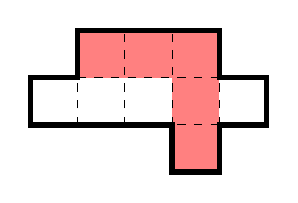
\begin{tikzpicture}[scale=0.6]
    \fill[red!50] (1,1) rectangle (4,2);
    \fill[red!50] (3,-1) rectangle (4,2);
    \draw[line width=2] (0,0)--(3,0)--(3,-1)--(4,-1)--(4,0)--(5,0)--(5,1)--(4,1)--(4,2)--(1,2)--(1,1)--(0,1)--cycle;
    \draw[dashed] (1,0) grid (4,2);
  \end{tikzpicture}
  \\~\\
  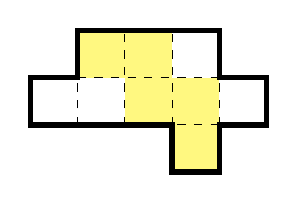
\begin{tikzpicture}[scale=0.6]
    \fill[yellow!50] (3,-1) rectangle (4,1);
    \fill[yellow!50] (2,0) rectangle (4,1);
    \fill[yellow!50] (2,0) rectangle (3,2);
    \fill[yellow!50] (1,1) rectangle (3,2);
    \draw[line width=2] (0,0)--(3,0)--(3,-1)--(4,-1)--(4,0)--(5,0)--(5,1)--(4,1)--(4,2)--(1,2)--(1,1)--(0,1)--cycle;
    \draw[dashed] (1,0) grid (4,2);
  \end{tikzpicture}
  \hspace{0.5cm}
  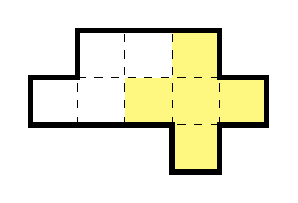
\begin{tikzpicture}[scale=0.6]
    \fill[yellow!50] (2,0) rectangle (5,1);
    \fill[yellow!50] (3,-1) rectangle (4,2);
    \draw[line width=2] (0,0)--(3,0)--(3,-1)--(4,-1)--(4,0)--(5,0)--(5,1)--(4,1)--(4,2)--(1,2)--(1,1)--(0,1)--cycle;
    \draw[dashed] (1,0) grid (4,2);
  \end{tikzpicture}
  \hspace{0.5cm}
  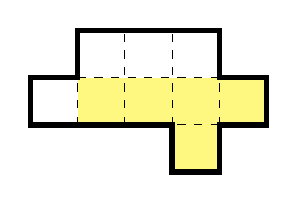
\begin{tikzpicture}[scale=0.6]
    \fill[yellow!50] (1,0) rectangle (5,1);
    \fill[yellow!50] (3,-1) rectangle (4,1);
    \draw[line width=2] (0,0)--(3,0)--(3,-1)--(4,-1)--(4,0)--(5,0)--(5,1)--(4,1)--(4,2)--(1,2)--(1,1)--(0,1)--cycle;
    \draw[dashed] (1,0) grid (4,2);
  \end{tikzpicture}
  \hspace{0.5cm}
  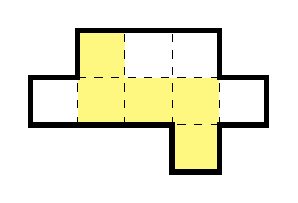
\begin{tikzpicture}[scale=0.6]
    \fill[yellow!50] (1,0) rectangle (2,2);
    \fill[yellow!50] (1,0) rectangle (4,1);
    \fill[yellow!50] (3,-1) rectangle (4,1);
    \draw[line width=2] (0,0)--(3,0)--(3,-1)--(4,-1)--(4,0)--(5,0)--(5,1)--(4,1)--(4,2)--(1,2)--(1,1)--(0,1)--cycle;
    \draw[dashed] (1,0) grid (4,2);
  \end{tikzpicture}
  \caption{
    A computer search has proven that a nine-cell region of the plane is the smallest
    possible region that contains all $5$-ominoes.
  }
\end{figure}
\begin{question}
  What is the smallest region of the plane (with respect to area) that can contain all free $n$-ominoes?
\end{question}

\begin{related}
  \item How about other polyforms?
  \item What about fixed polyominoes? One-sided polyominoes (those that can be rotated but not flipped)?
  \item What about other polyforms such as polyhexes or polycubes?
  \item How many distinct minimal covering sets (call this $c(n)$)?
  \item What if the region must be convex?
  \item What is the asymptotic growth in area of such a region? (Somewhere between linear and quadratic.)
  \item Is there a limiting shape?
  \item Alec Jones wonders if there always exists a covering set such that a single
    cell is used by all polyominoes.
\end{related}

\begin{note}
  If $c(n)$ counts the number of distinct minimal covering sets of $n$-ominoes,
  then $c(1) = c(2) = c(3) = 1$, $c(4) = c(5) = 2$, and $c(6) = 14$.
\end{note}

\begin{references}
  \item Problem 85
  \item \url{https://en.wikipedia.org/wiki/Moser%27s_worm_problem}
  \item \url{https://math.stackexchange.com/q/2831675/121988}
\end{references}
\end{document}

% a(6) = 12
% #
% ####
% ######
%   #
%
% a(7) <= 17
% #
% #####
% #######
%  ###
%   #
%
% a(8) <= 22
%   ##
% ####
%   ###
%   ###
%  #####
%    ##
%    #
%   ##
%
% a(9) <= 26
%   #####
% #########
% #######
%  ###
%   ##
%
%
% a(10) <= 32
%  ###
% #####
% #####
% #####
% ### #
% ###
% ###
%  #
%  #
%  ##
